\chapter[Gerência de Requisitos]{Gerência de Requisitos}

\section{Nível de Portifólio}

A camada de Portfólio consiste no nivel mais elevado do SAFe, onde programas sao alinhados à
estratégia de negócios da empresa ao longo de linhas da corrente de valor. No presente trabalho,
o nivel de portfólio é destacado a partir das atividades \textbf{Entender o Contexto do Cliente},
\textbf{Levantar Epicos} e \textbf{Selecionar e detalhar épicos} que foram realizadas utilizando as
técnicas de elicitação, workshops e entrevistas. As atas de reunião, jutamente com as entrevistas,
podem ser encontradas no apêndice (COLOCAR O NUMERO DO APENCIE).

\subsection{Requisitos Identificados}

\textbf{Tema de Investimento:} Gestão da Manutenção

Extraido a partir das prioridades da organização, serve para assegurar que o desenvolvimento
do software estará de acordo com a estrategia da organização.

Dado que o gargalo identificado na gestão da manutenção de sistemas do MC e onde o cliente irá investir.
Cada épico foi detalhado utilizando o template de lightweight business case, recomendado pelo SAFe. \cite{scaleP}

\textbf{Épico 01:} EP-01 Gerenciamento de Demandas

Abrange todo o movimento das demandas em torno do fluxo estabelecido, desde sua criacao ate o seu fechamento.

\begin{table}[]
\centering
\caption{Épico 1}
\label{my-label}
\begin{tabular}{|c|c|}
\hline
\multicolumn{2}{|c|}{Caso de Negócio}                                                                                                                \\ \hline
Para                 & O gerente e a equipe de desenvolvimento                                                                                       \\ \hline
Quem                 & Gere e desenvolve as demandas aprovadas de manutenção do ministério                                                           \\ \hline
A                    & Ferramenta de Gestão do Desenvolvimento                                                                                       \\ \hline
É uma                & Ferramenta que organiza sistematicamente a demanda a ser desenvolvida                                                         \\ \hline
Que                  & Facilita e Agiliza o trabalho da equipe de desenvolvimento                                                                    \\ \hline
Diferente            & Da situação atual que tudo é feito manualmente                                                                                \\ \hline
Nossa Soluação       & Automatiza a gestão e Centraliza as informações das demandas a serem desenvolvidas                                            \\ \hline
\multicolumn{2}{|c|}{Escopo}                                                                                                                         \\ \hline
Critérios de Sucesso & \begin{tabular}[c]{@{}c@{}}Produtividade aumentar em 100\%\\ \\ Demandas aprovadas pelo usuário aumentar em 20\%\end{tabular} \\ \hline
No Escopo            & Controle de demandas por parte do Gestor.                                                                                     \\ \hline
Fora do Escopo       & \begin{tabular}[c]{@{}c@{}}Validação de demandas.\\ Registro de demanda por parte do cliente.\end{tabular}                    \\ \hline
\end{tabular}
\end{table}

\textbf{Épico 02:} EP-02 Gerenciamento de Usuários

Interfere no modo de comunicacao entre o usuario e o sistema, considerando diversos aspectos referente ao seu acesso.

\begin{table}[H]
\centering
\caption{Épico 2}
\label{epic:segundo}
\begin{tabular}{|c|c|}
\hline
\multicolumn{2}{|m{4cm}|}{\textbf{Caso de Negócio}} \\ \hline
  Para   &   O gerente e a equipe de desenvolvimento        \\ \hline
  Quem         &    Gere e desenvolve as contas de usuário        \\ \hline
    A       &     Ferramenta de Gestão do Manutenção    \\ \hline
      É uma     &    Ferramenta que organiza sistematicamente a demanda a ser desenvolvida \\ \hline
      Que     &     Facilita e Agiliza o trabalho da equipe de desenvolvimento \\ \hline
      Diferente   &     Da situação atual que tudo é feito manualmente     \\ \hline
      Nossa Soluação  &   Automatiza a gestão e Centraliza as informações das demandas a serem desenvolvidas    \\ \hline
\multicolumn{2}{|l|}{Escopo} \\ \hline
Critérios de Sucesso  &  Produtividade aumentar em 100\% e Demandas aprovadas pelo usuário aumentar em 20\%    \\ \hline
No Escopo & Controle de demandas por parte do Gestor. \\ \hline
Fora do Escopo  & Validação de demandas. e Registro de demanda por parte do cliente.     \\ \hline
\end{tabular}
\end{table}



\section{Nível de Programa}

A camada de Programa consiste na camada intermediária do SAFe, onde tem uma relação
direta com o nível de time e o planejamento das iterações. No presente trabalho,
o nivel de programa foram executadas as seguintes atividades: eh destacado a partir das atividades:

\begin{itemize}
  \item Leventar Requisitos não funcionais
  \item Selecionar épicos para iteração,
  \item Levantar features
  \item Levantar histórias de usuário
  \item Planejar Releases
  \item Gerenciar Mudanças
\end{itemize}


\subsection{Requisitos não funcionais}

Os requisitos não funcionais identificados se encontram no documento de visão que se encontra no apendice
[apendice]. Neles foram especificadas regras como níveis de usuário de acesso entre outras restrições
que contribuiram também para elicitar os requisitos da próxima sessão.

\subsection{Requisitos identificados}

Considerando as atividades do processo, foram levantadas as features e suas
respectivas histórias, para obter uma melhor estimativa no planejamento das releases,
nesta sessão serão descritas apenas as features levantadas, as histórias se encontram

\textbf{Feature 1:} Manutenção de Usuários

Esta feature tem como objetivo manter os usuários do sistema, permitindo o cadastro,
definição de tipo de conta, cadastro de usuários e edição dos mesmos.

\textbf{Feature 2:} Acesso de Usuários

Essa feature tem como objetivo o controle da sessão dos usuários permitindo os
mesmos se `logar` no sistema e recuprar sua senha.


\textbf{Feature 3:} Acompanhamento de Demandas
Essa feature tem como objetivo prover as funcionalidades para
que os stakeholders consigam acompanhar as demandas e visualizar
as mesmas de acordo com o seu nível de usuário.


\textbf{Feature 4:} Manutenção de Demandas
Essa feature tem com oobjetivo a manutenção das demandas e atualização das
demandas seguindo o workflow de trabalho da equipe de manutenção. Proverá
a possibilidade de mudar status e responsável sobre as demandas.

\subsection{Visão}

Você deve pensar sobre grandes coisas enquanto você está fazendo coisas pequenas, garantindo que
todas as pequenas coias estão indo na direção certa
\cite{alvin}. Uma frase detalhada na descrição do documento de visão no SAFe,
que, descreve o Documento de visão como um documento que descreve uma explanação sobre a
solução a ser desenvolvida, com os requisitos não funcionais, necissdads dos stakeholders e
um resumo do contexto do sistema. O documento de visão produzido se encontra no apêndice \ref{apendices:visao}
e foi bem utilizado como passo para as próximas atividades.

\subsection{Roadmap}

O Roadmap serve como um documento que padroniza a comunicação entre o nível de time o programa,
é como um caminho que deve ser seguido em uma linha do tempo das entregas que devem ser realizadas.
Representa de 3 a 6 meses de Iterações. Representa os incrementos do software que devem ser entregues.
Existem dois tipos de Roadmap: \cite{scaleR}

\begin{itemize}
  \item \textbf{síncrono:} features são entregue sincronizadas, em cada release é entregue uma feature completa.
  \item \textbf{asincrono:} features são entregues por versões, uma release não precisa conter uma feature completa,
   mas sim uma versão que pode ser incrementada, na próxima release.
\end{itemize}

O planejamento atual, foi realizado usando o roadmap asincrono, como representado na imagem abaixo

\begin{figure}[H]
    \centering
	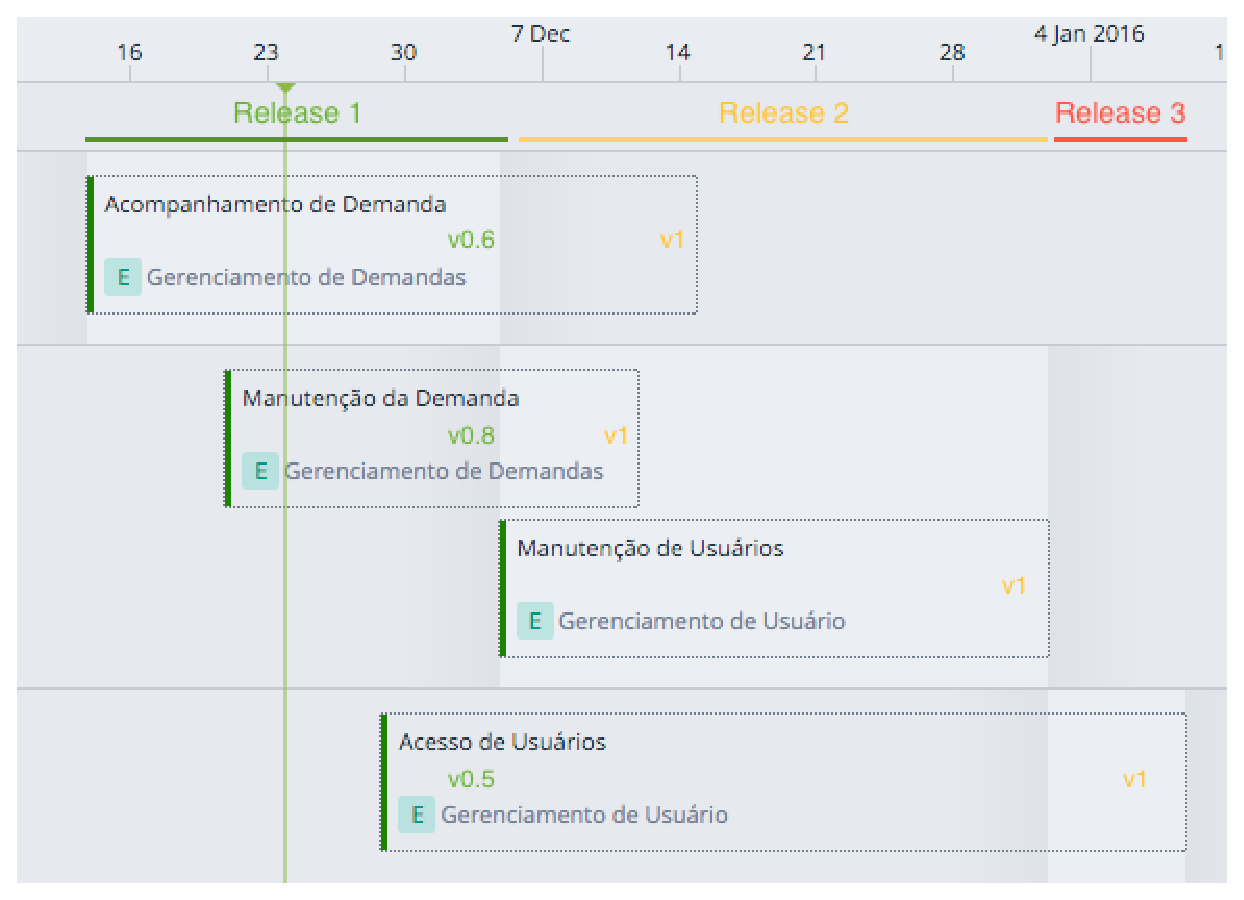
\includegraphics[keepaspectratio=true,scale=0.5]{figuras/roadmap.eps}
    \caption{Roadmap planejado}
    \label{fig:roadmap}
\end{figure}

Como descrito na imagem ,a Feature \"Acompanhamento de demenda\", na release 1.
será lançada uma v0.6 com 60\% das suas funcionalidades implementadas e a versão
final será entregue na Release 2. Respectivamente aconterá o mesmo com as outras features.

\section{Nível de Time}

\section{Gerência de Requisitos}

\subsection{Atributos de Requisitos}

\subsection{Rastreabilidade de Requisitos}
